% referee sugg: laczny, iqbal
% @CTB discuss inclusion rather than accuracy
% @CTB should we talk about 500bp cutoff?
% @CTB make point about sequencing individual colonies in a mock?
% @CTB comment re metaspades vs spades
% @CTB comment re megahit / high coverage / performing worse

%%%%%%%%%%%%%%%%%%%%%%%%%%%%%%%%%%%%%%%%%%%%%%%%%%%%%%%%%%%%%%%
%
% Welcome to Overleaf --- just edit your article on the left,
% and we'll compile it for you on the right. If you give 
% someone the link to this page, they can edit at the same
% time. See the help menu above for more info. Enjoy!
%
%%%%%%%%%%%%%%%%%%%%%%%%%%%%%%%%%%%%%%%%%%%%%%%%%%%%%%%%%%%%%%%
%
% For more detailed article preparation guidelines, please see:
% http://f1000research.com/author-guidelines

\documentclass[11pt]{article}
%% Default: numerical citations
\usepackage[numbers]{natbib}
\usepackage{graphicx}
\usepackage{lineno}
\linenumbers

\setlength{\parskip}{0.2em}

%% Uncomment this lines for superscript citations instead
% \usepackage[super]{natbib}

%% Uncomment these lines for author-year citations instead
% \usepackage[round]{natbib}
% \let\cite\citep

\begin{document}

\title{Evaluating Metagenome Assembly on a Simple Defined Community with Many Strain Variants}

\author{Sherine Awad$^{1}$, Luiz Irber$^{1}$, C. Titus Brown$^{1\ast}$\\
\small
\bf{$^1$}Department of Population Health and Reproduction \\
\small
University of California, Davis\\
\small
Davis, CA 95616 USA\\
\small
$\ast$ E-mail: ctbrown@ucdavis.edu
} 

\maketitle
%\thispagestyle{fancy}

% Please list all authors that played a significant role in the research involved in the article. Please provide full affiliation information (including full institutional address, ZIP code and e-mail address) for all authors, and identify who is/are the corresponding author(s).

\begin{abstract}
 
  We evaluate the performance of three metagenome assemblers, IDBA,
  MetaSPAdes, and MEGAHIT, on short-read sequencing of a defined ``mock''
  community containing 64 genomes (Shakya et al. (2013)).  We update
  the reference metagenome for this mock community and detect several
  additional genomes in the read data set.  We show that strain
  confusion results in significant loss in assembly of reference
  genomes that are otherwise completely present in the read data set.
  In agreement with previous studies, we find that MEGAHIT performs
  best computationally; we also show that MEGAHIT tends to recover
  larger portions of the strain variants than the other assemblers.
  
\end{abstract}

\clearpage

\section*{Introduction}

Metagenomics refers to sequencing of DNA from a mixture of organisms,
often from an environmental or uncultured sample. Unlike whole genome
sequencing, metagenomics targets a mixture of genomes, which
introduces metagenome-specific challenges in analysis
\cite{ghurye2016metagenomic}.  Most approaches to analyzing
metagenomic data rely on mapping or comparing sequencing reads to
reference sequence collections. However, reference databases contain
only a small subset of microbial diversity \cite{geba}, and much
of the remaining diversity is evolutionarily distant and search
techniques may not recover it \cite{CAMI}.

As sequencing capacity increases and sequence data is generated from
many more environmental samples, metagenomics is increasingly using
{\em de novo} assembly techniques to generate new reference genomes
and metagenomes \cite{Sharon2012}.  There are a number of metagenome
assemblers that are widely used - see \cite{Vollmers2017} for an
overview of the available software, and \cite{ghurye2016metagenomic}
for a review of the different assembler methodologies. However,
evaluating the results of these assemblers is challenging due to the
general lack of good quality reference metagenomes.

%-----------Literature Review starts here ---------------------

Moya et al. in \cite{moya2014} evaluated metagenome assembly using
two simulated 454 viral metagenome and six assemblers. The assemblies
were evaluated based on several metrics including N50, percentages of
reads assembled, accuracy when compared to the reference genome. In
addition to, chimeras per contigs and the effect of assembly on
taxonomic and functional annotations.
 
Mavromatis et al. in \cite{mavromatis2007} provided a benchmark study
to evaluate the fidelity of metagenome processing methods. The study used
simulated metagenomic data sets constructed at different complexity
levels.
The datasets were assembled using Phrap v3.57, Arachne v.2
\cite{arachne} and JAZZ \cite{jazz}.
This study evaluates assembly, gene prediction, and binning
methods. However, the study did not evaluate the assembly quality
against a reference genome.

Rangwala et al. in \cite{huzefa2011} presented an evaluation study of
metagenome assembly. The study used a de Bruijn graph based assembler
ABYSS \cite{abyss} to assemble simulated metagenome reads of 36 bp. The
data set is classified at different complexity levels.  The study
compared the quality of the assembly of the data sets in terms of
contig length and assembly accuracy. The study also took into
consideration the effect of kmer size and the degree of chimericity.
However, the study evaluated the assembly based on only one
assembler. Also, both previous studies used simulated data, which may
lack confounders of assembly such as sequencing artifacts and GC bias.

In a landmark study, Shakya et al. (2013) constructed a synthetic
community of organisms by mixing DNA isolated from individual cultures
of 64 bacteria and archaea, including a variety of strains across a
range of nucleotide distances \cite{podar}.  In addition to performing
16s amplicon analysis and doing 454 sequencing, the authors
shotgun-sequenced the mixture with Illumina.  While the authors
concluded that this metagenomic sequencing generally outperformed
amplicon sequencing, they did not conduct an assembly based analysis.
This data set was also used in several other evaluation studies,
including gbtools for binning \cite{Seah2015} and benchmarking of the
MEGAHIT assembler \cite{Li2016}.

% @CTB pignatelli & moya 2011

More recently, several benchmark studies systematically evaluated
metagenome assembly of short reads.  The Critical Assessment of
Metagenome Interpretation (CAMI) collaboration benchmarked a number of
metagenome assemblers on several data sets of varying complexity,
evaluating recovery of novel genomes and multiple strain variants
\cite{CAMI}.  Notably, CAMI concluded that ``The resolution of
strain-level diversity represents a substantial challenge to all
evaluated programs.''  Another recent study evaluated eight assemblers
on nine environmental metagenomes and three simulated data sets and
provided a workflow for choosing a metagenome assembler based on the
biological goal and computational resources available
\cite{metag_one}.  \cite{Vollmers2017} explored metagenome assembler
performance on a pair of real data sets, again concluding that the
biological goal and computational resources defined the choice of
assembler.  Also see \cite{Greenwald2017} for an analysis of a previously
generated HMP benchmark data set; however, the Illumina reads used for this
study are much shorter than current sequencing and are arguably not relevant
for future studies.

In this study, we extend previous work by delving into questions of
chimeric misassembly and strain recovery in the Shakya et al. (2013)
data set.  First, we update the list of reference genomes for Shakya
et al. to include the latest GenBank assemblies along with
plasmids. We then compare IDBA \cite{idba}, MetaSPAdes \cite{metaspades},
and MEGAHIT \cite{megahit} performance on assembling this short-read
data set, and explore concordance in recovery between the three
assemblers.  We describe the effects of ``strain confusion'' between
multiple strains.  We also detect and analyze several previously
unreported strains and genomes in the Shakya et al. data set.  We find
that in the absence of closely related genomes, all three metagenome
assemblers recover 95\% or more of known reference genomes.  However,
in the presence of closely related genomes, these three metagenome
assemblers vary widely in their performance and, in extreme cases, can
fail to recover the majority of some genomes even when they are
completely present in the reads.  Our report provides strong guidance
on choice of assemblers and extends previous analyses of this
low-complexity metagenome benchmarking data set.

% \subsection*{Sections}

% Use section and subsection commands to organize your document. \LaTeX{} handles all the formatting and numbering automatically. Use ref and label commands for cross-references.


% Removed this line for now \subsection*{Tables}

% Use the table and tabledata commands for basic tables --- see Table~\ref{tab:widgets}, for example.
% \begin{table}[h!]
% \hrule \vspace{0.1cm}
% \caption{\label{tab:widgets}An example of a simple table with caption.}
% \centering
% \begin{tabledata}{llr} 
% \header First name & Last Name & Grade \\ 
% \row John & Doe & $7.5$ \\ 
% \row Richard & Miles & $2$ \\ 
% \end{tabledata}
% \end{table}
 
%-----------------------------Misassembles table 

 
%\begin{figure}[!h]
%\centering
%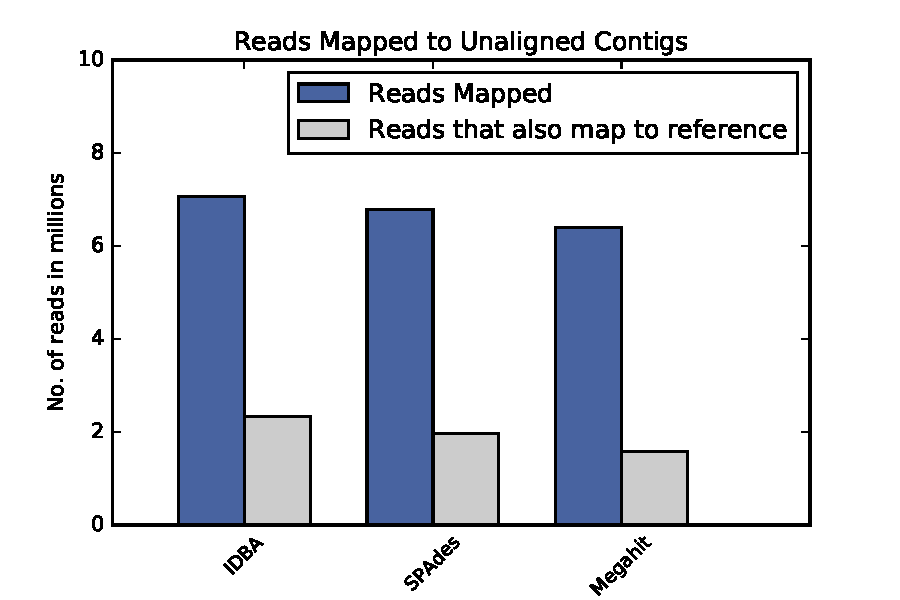
\includegraphics[width=0.45\textwidth]{UnalignmentHistogram.pdf} %to be changed to qc.coverage-profile
%\caption{Mapping unaligned reads to reference genome using identity 99\%, and Ambiguous Approach CTB This can't be right :)}
%\label{fig:unaligned-reads}
%\end{figure}

% \begin{figure}[!ht]
% \centering
% 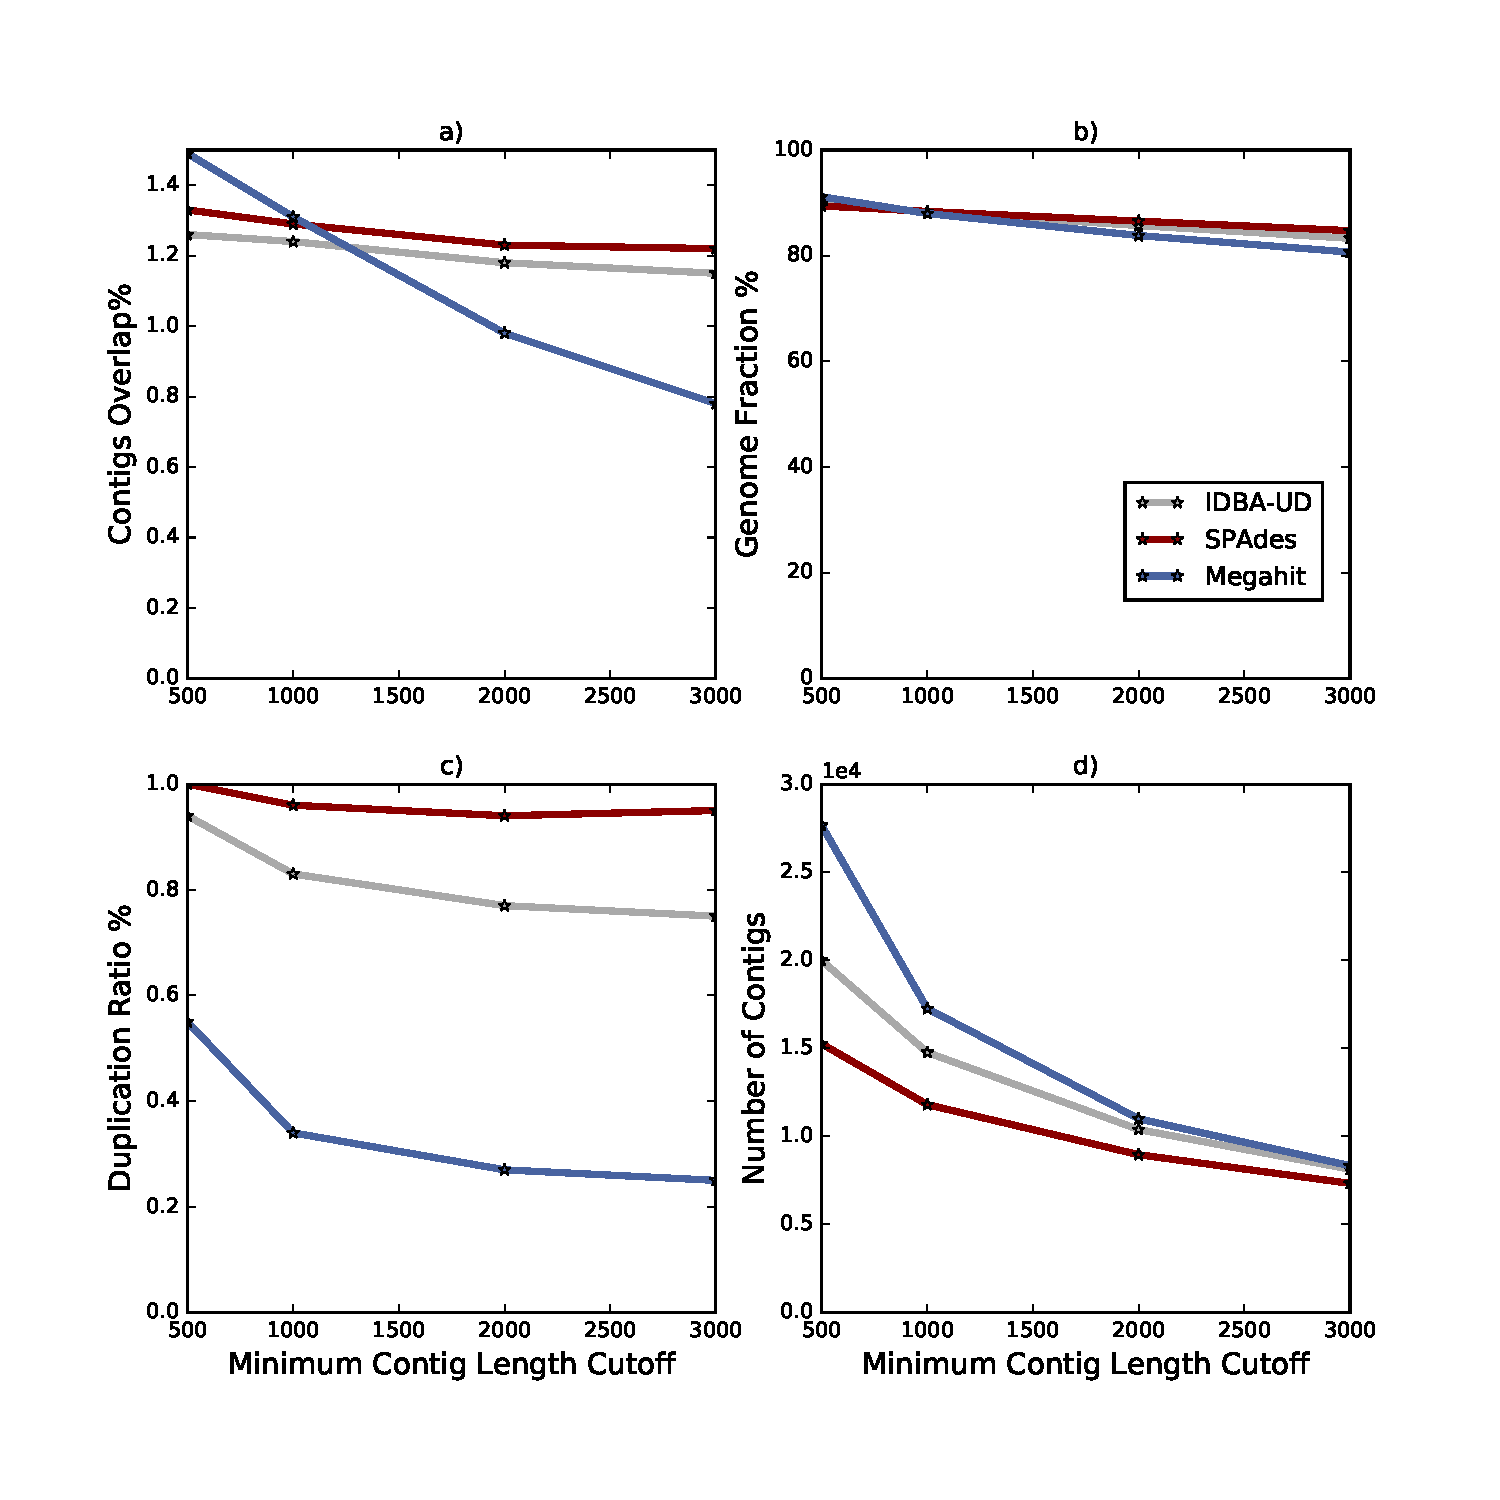
\includegraphics[width=9.5cm,height=9.5cm]{min-contig-analysis.pdf}  
% \caption{\label{fig:min-contig-analysis} Genome fraction, duplication ratio, Contigs overlap ratio, and number of contigs using different minimum contig length,  identity 99\%, and Ambiguous Approach}
% \end{figure}

% CTB maybe we should put this back in?
% \begin{figure}[!h]
% \centering
% 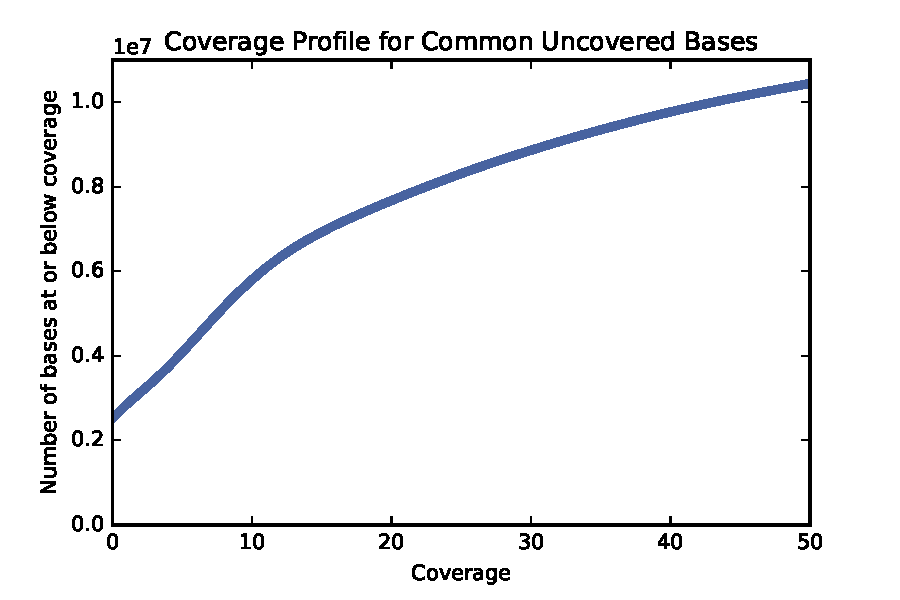
\includegraphics[width=0.4\textwidth]{CommonUncoveredCoverageProfile.pdf} 
% \caption{Cumulative read coverage for bases in the reference metagenome missing from all three assemblies.}
% \label{fig:CommonUncovered}
% \end{figure}



% \begin{figure}[!h]
% \centering
% \includegraphics[width=0.4\textwidth]{MapQuality.png}  
% \caption{\label{fig:mapquality} Mapping Quality for Quality Filtered Reads to the Reference Genome}
% \end{figure}

% \begin{figure}[!h]
% \centering
% \includegraphics[height=2.6cm,width=0.4\textwidth]{basequality.png}  
% \caption{\label{fig:basequality} Mean Base Quality}
% \end{figure}

% \begin{figure}[!h]
% \centering
% \includegraphics[height=2.6cm, width=0.4\textwidth]{errorprofile30.png}  
% \caption{\label{fig:errorprofile30}Error Profiles for MAPQ >=30}
% \end{figure}

% \begin{figure}[!h]
% \centering
% \includegraphics[height=2.6cm, width=0.4\textwidth]{nucleotidecomposition.png}  
% \caption{\label{fig:nucleotidecomposition.png}Nucleotide Composition for MAPQ >=30}
% \end{figure}
% \subsection*{Mathematics}

 
% \subsection*{Mathematics}

\subsection*{Datasets}
%Numbers in this section are up to date 22 december 2016

We used a diverse mock community data set constructed by pooling DNA
from 64 species of bacteria and archaea and sequencing them with
Illumina HiSeq.  The raw data set consisted of 109,629,496 reads from
Illumina HiSeq 101 bp paired-end sequencing (2x101) with an untrimmed
total length of 11.07 Gbp and an estimated fragment size of 380 bp
\cite{podar}.
 
The original reads are available through the NCBI Sequence Read
Archive at Accession SRX200676.  We updated the 64 reference genomes
sets from NCBI GenBank using the latest available assemblies with
plasmid content (June 2017); the accession numbers are available as
{\tt accession-list-ref.txt} in the Zenodo repository, DOI:
10.5281/zenodo.821919.
For convenience, the updated reference genome collection is
available for download at the archival URL https://osf.io/vbhy5/.

\section*{Methods}

The analysis code and run scripts for this paper are written in Python
and bash, and are available at
https://github.com/dib-lab/2016-metagenome-assembly-eval/ (archived at
Zenodo DOI: 10.5281/zenodo.821919). The scripts and overall
pipeline were examined by the first and senior authors for
correctness.  In addition, the bespoke reference-based analysis
scripts were tested by running them on a single-colony {\em E. coli}
MG1655 data set with a high quality reference genome
\cite{chitsaz2011}.

\subsection*{Quality Filtering} 

We removed adapters with Trimmomatic v0.30 in paired-end mode with the
TruSeq adapters \cite{trimmomatic}, using light quality score trimming
({\tt LEADING:2 TRAILING:2 SLIDINGWINDOW:4:2 MINLEN:25})
as recommended in MacManes, 2014 \cite{macmanes2014optimal}.

\subsection*{Reference Coverage Profile}

To evaluate how much of the reference metagenome was contained in the
read data, we used {\tt bwa aln} (v0.7.7.r441) to map reads to the
reference genome \cite{bwa}.  We then calculated how many reference
bases were covered by mapped reads (custom script {\tt
  coverage-profile.py}).

% Makefile target: readcoverage

\subsection*{Measuring k-mer inclusion and Jaccard similarity}

We used MinHashing as implemented in sourmash to estimate k-mer
inclusion and Jaccard similarity between data sets \cite{sourmash}.
MinHash signatures were prepared with {\tt sourmash compute} using
{\tt --scaled 10000}.  K-mer inclusion was computed by taking the ratio of
the number of intersecting hashes with the query over the total number
of hashes in the subject MinHash. Jaccard similarity was computed as
in \cite{mash} by taking the ratio of the number of intersecting
hashes between the query and subject over the number of hashes in the
union.  K-mer sizes for comparison were chosen at 21, 31, or 51,
depending on the level of taxonomic specificity desired - genus,
species, or strain, respectively, as described in \cite{metapalette}.

% Makefile target: sigs

Where specified, high-abundance k-mers were selected for counting by
using the script {\tt trim-low-abund.py} script with {\tt -C 5} from
khmer v2 \cite{streaming, khmer2}.

% Makefile target: SRR606249-hardtrim

\subsection*{Assemblers}

We assembled the quality-filtered reads using three different
assemblers: IDBA-UD \cite{idba}, MetaSPAdes \cite{metaspades}, and MEGAHIT
\cite{megahit}.  For IDBA-UD v1.1.1 \cite{idba}, we used {\tt
  {--pre\_correction}} to perform pre-correction before assembly and
-r for the pe files.  IDBA could not ingest the single-ended files so
they were omitted from the assembly.

% Makefile target: idba-quality-assembly500.fa

For MetaSPAdes v3.10.1 \cite{metaspades}, we used { \tt {--meta --pe1-12
    --pe1-s}} where {\tt{--meta}} is used for
metagenomic data sets, {\tt{--pe1-12}} specifies the interlaced reads
for the first paired-end library, and {\tt{--pe1-s}} provides the
orphan reads remaining from quality trimming.

% Makefile target: spades-quality-assembly500.fa

For MEGAHIT v1.1.1-2-g02102e1 \cite{megahit}, we used -l 101 {\tt{-m 3e9
    --cpu-only}} where {\tt -l} is for maximum read length, {\tt -m} is
for max memory in bytes to be used in constructing the graph, and {\tt
  {--cpu-only}} to use only the CPU and no GPUs. We also used {\tt
  {--presets meta-large}} for large and complex metagenomes, and {\tt
  {--12} } and {\tt{-r}} to specify the
interleaved-paired-end and single-end files respectively.  MEGAHIT allows
the specification of a memory limit and we used {\tt -M 1e+10} for 10 GB.

% Makefile target: megahit-quality-assembly500.fa

All three assemblies were executed on the same XSEDE Jetstream
instance (S1.Xxlarge) at Indiana University, running Ubuntu 16.04
(install 6/21/17, Ubuntu 16.04 LTS Development + GUI support + Docker;
based on Ubuntu cloud image for 16.04 LTS with basic dev tools,
GUI/Xfce added).  Assemblers were limited to 16 threads.  We recorded
RAM and CPU time for each assembly using {\tt /usr/bin/time -v}.
Install and execute details as well as output timings and logs are
available in the {\tt pipeline/runstats} directory of the Zenodo
release.

Unless otherwise mentioned, we eliminated all contigs less than 500 bp
from each assembly prior to further analysis.

\subsection*{Mapping}

We aligned all quality-filtered reads to the reference metagenome with
bwa aln (v0.7.7.r441) \cite{bwa}. We aligned paired-end and orphaned
reads separately. We then used samtools (v0.1.19)
\cite{sam-stools} to convert SAM files to BAM files for both
paired-end and orphaned reads. To count the unaligned reads, we
included only those records with the ``4'' flag in the SAM files
\cite{sam-stools}.
 
\subsection*{Assembly analysis using NUCmer}

We used the NUCmer tool from MUMmer3.23 \cite{mummer3.0} to align
assemblies to the reference genome with options {\tt \--coords} {\tt
  -p}. Then we parsed the generated ``.coords'' file using a custom
script {\tt{analyze\_assembly.py}}, and calculated several analysis
metrics across all three assemblies at a 99\% alignment identity.

% Makefile target: mqc500.coords assemblies.stats.QC.AMBIGUOUS.99

\subsection*{Reference-based analysis of the assemblies}

We conducted reference-based analysis of the assemblies under two
conditions.  ``Loose'' alignment conditions used all available
alignments, including redundant and overlapping alignments. ``Strict''
alignment conditions took only the longest alignment for any given
contig, eliminating all other alignments.

% see Makefile target above, assemblies.stats.QC.AMBIGUOUS.99 (loose) and
% assemblies.stats.QC.BESTHIT.99 (strict)

The script {\tt summarize-coords2.py} was used to calculate aligned
coverage from the loose alignment conditions: each base in the reference
was marked as ``covered'' if it was included in at least one alignment.
The script {\tt analyze\_ng50.py} was used to calculate NGA 50 for
each individual reference genome.

% Makefile target: nga50

\subsection*{Analysis of chimeric misassemblies}

%CTB cami, disco used quast.

We analyzed each assembly for chimeric misassemblies by counting the
number of contigs that contained matches to two distinct reference
genomes.  In order to remove secondary alignments from consideration,
we included only the longest non-overlapping NUCmer
alignments for each contig at a minimum alignment identity of 99\%.
We then used the script {\tt analyze\_chimeric2.py} to find individual
contigs that matched more than one distinct reference genome.  As a
negative control on our analysis, we verified that this approach
yielded no positive results when applied to the alignments of the
reference metagenome against itself.

% Makefile target: chimera.sqc50k.txt

\subsection*{Analysis of unmapped reads}

We conducted assembly and analysis of unmapped reads with MEGAHIT,
NUCmer, and sourmash as above.  The new GenBank genomes are listed in
the Zenodo archive at the file {\tt accession-list-unmapped.txt} and
for convenience are available for download at the archival URL
https://osf.io/34ef8/.

\section*{Results}

\subsection*{The raw data is high quality.}

The reads contains 11,072,579,096 bp (11.07 Gbp) in 109,629,496 reads
with 101.0 average length (2x101bp Illumina HiSeq).

Trimming removed 686,735 reads (0.63\%).  After trimming, we retained
108,422,358 paired reads containing 10.94 Gbp with an average length of
100.9 bases. A total of 46.56 Mbp remained in 520,403 orphan reads with
an average length of 89.5 bases. In total, the quality trimmed data
contained 10.98 Gbp in 108,942,761 reads.  This quality trimmed (``QC'')
data set was used as the basis for all further analyses.
% These numbers are calculated using readstats from khmer

\begin{figure}[!h]

% notebooks/coverage-profile.ipynb
  
\centering
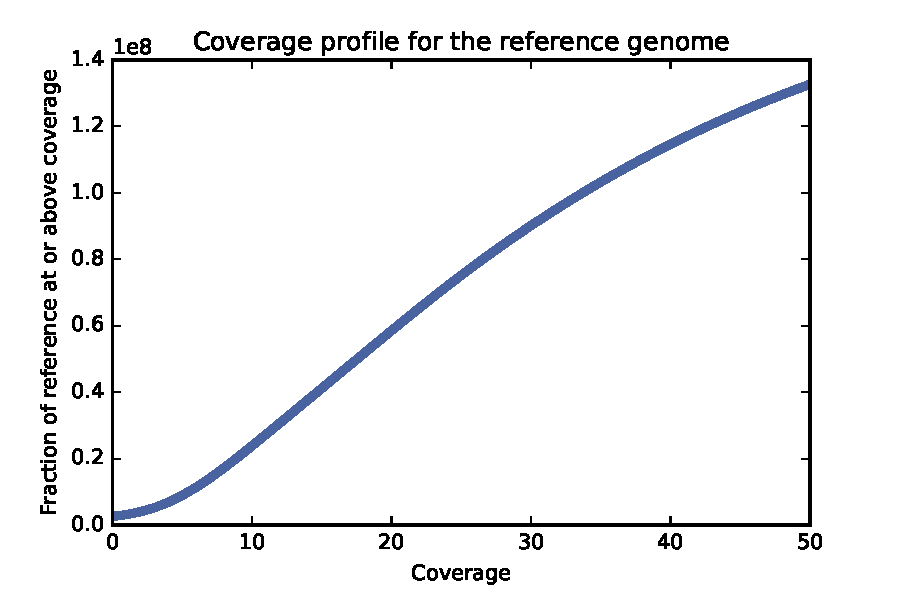
\includegraphics[width=0.45\textwidth]{CoverageProfile.pdf}  
\caption{\label{fig:coverage-profile} Cumulative coverage profile for the reference metagenome, based on read mapping. }
\end{figure}

\subsection*{The reference metagenome is not completely present in the reads.}

We next evaluated the fraction of the reference genome covered by at least
one read (see Methods for details). Quality filtered reads cover
203,058,414 (98.76\%) bases of the reference metagenome (205,603,715
bp total size).  Figure \ref{fig:coverage-profile} shows the
cumulative coverage profile of the reference metagenome, and the
percentage of bases with that coverage. Most of the reference
metagenome was covered at least minimally; only 3.33\% of the
reference metagenome had mapping coverage \textless 5, and 1.24\% of
the bases in the reference were not covered by any reads in the QC data
set.

\begin{table}[t]
\caption{Jaccard containment of the reference in the reads}
\centering
\begin{tabular}{|c|c|}
\hline
\textbf{k-mer size} & {\textbf \% reference in reads } \\ [0.5ex]
\hline
21 & 96.8\% \\
\hline
31 & 95.9\% \\
\hline
41 & 94.9\% \\
\hline
51 & 94.1\% \\
\hline
\end{tabular}
\label{table:ref_in_reads}
\end{table}

In order to evaluate reconstructability with De Bruijn graph
assemblers, we next examined k-mer containment of the reference in the
reads for $k$ of 21, 31, 41, and 51 (Table \ref{table:ref_in_reads}).
The k-mer overlap decreases from 96.8\% to 94.1\% as the k-mer size
increases. This could be caused by low coverage of some portions
of the reference and/or variation between the reads and the reference.

\subsection*{Some individual reference genomes are poorly represented in the reads.}

% measured in *.cov.txt

\begin{table}[!h]
\centering
\caption{Top uncovered genomes}
\begin{tabular}{|l|c|c|}\hline
\textbf{Genome} & \textbf {Read coverage} \\ \hline 

%genomes/17.fa.cov.sam 0.931870428479 3411942.0 3661391.0
%>NC_008751.1 Desulfovibrio vulgaris DP4, complete genome
%82.5
{{\em Desulfovibrio vulgaris} DP4}  & 93.2\% \\
\hline
%genomes/55.fa.cov.sam 0.910651720402 1725573.0 1894877.0
%>AE017221.1 Thermus thermophilus HB27, complete genome
%79.7
{{\em Thermus thermophilus} HB27}  & 91.1\% \\
\hline
%genomes/19.fa.cov.sam 0.746209918949 2510480.0 3364308.0
%>NZ_KE136524.1 Enterococcus faecalis V583 acyDH-supercont2.1, whole genome shotgun sequence
%65.6
{{\em Enterococcus faecalis} V583}  & 74.6\% \\
\hline
%genomes/20.fa.cov.sam 0.475837203955 1034708.0 2174500.0
%>AE009951.2 Fusobacterium nucleatum subsp. nucleatum ATCC 25586, complete genome
%18.2
{{\em Fusobacterium nucleatum}}  & 47.6\% \\
\hline
\end{tabular}
\label{table:genomes_uncovered-analysis}
\end{table}

To see if specific reference genomes exhibited low coverage, we
analyzed read mapping coverage for individual genomes.  Of the 64
reference genomes used in the metagenome, 60 had a per-base mapping
coverage above 95\%.  The remaining four varied significantly
(Table~\ref{table:genomes_uncovered-analysis}), with {\em
  F. nucleatum} the lowest -- only 47.6\% of the bases in the
reference genome are covered by one or more mapped reads.

\begin{table}[t]
\caption{Genomes removed from reference for low 51-mer presence}
\centering
\begin{tabular}{|c|l|}
\hline

\textbf{51-mers in reads}& \textbf{Genome} \\ [0.5ex] % inserts table %heading
\hline
98.7 & { \small \em Leptothrix cholodnii } \\ \hline
98.7 & { \small \em Haloferax volcanii} DS2  \\ \hline
98.6 & { \small \em Salinispora tropica} CNB-440 \\ \hline
97.4 & { \small \em Deinococcus radiodurans } \\ \hline
97.2 & { \small \em Zymomonas mobilis } \\ \hline
97.1 & { \small \em Ruegeria pomeroyi } \\ \hline
96.8 & { \small \em Shewanella baltica} OS223  \\ \hline
95.5 & { \small \em B. bronchiseptica} D989  \\ \hline
94.5 & { \small \em Burkholderia xenovorans } \\ \hline
72.0 & { \small \em Desulfovibrio vulgaris} DP4  \\ \hline
65.0 & { \small \em Thermus thermophilus} HB27  \\ \hline
53.4 & { \small \em Enterococcus faecalis } \\ \hline
4.7 & { \small \em Fusobacterium nucleatum} ATCC 25586  \\ \hline
\end{tabular}
\label{table:51mer_remove}
\end{table}

% new reference size: 141,394,815

We next did a 51-mer containment analysis of each reference genome in
the reads; k=51 was chosen so as to be specific to strain content
\cite{metapalette}.  99\% or more of the constituent 51-mers for 51 of
the 64 reference genomes were present in the reads, suggesting that
each of the 51 genomes was entirely present at some minimal coverage.

We excluded the remaining 13 genomes (see
Table~\ref{table:51mer_remove}) from any further reference-based
analysis because interpreting recovery and misassembly statistics for
these genomes would be confounding; also see the discussion of strain
variants, below.

\subsection*{MEGAHIT is the fastest and lowest-memory assembler evaluated}
%Numbers in this section are up to date 22 december 2016

 %------------------------------------Cost of Assembly ---------------
 \begin{table}[h]
\caption{Running Time and Memory Utilization}
\centering
\begin{tabular}{|l|c|c|c|}
\hline
\textbf{Assembler} & \textbf{CPU time} & \textbf{Wall time} & \textbf{RAM (Max RSS)} \\ [0.5ex]
\hline
MEGAHIT & 1191m & 1h 33m & 10 GB \\
\hline
IDBA-UD & 2117m & 2h 41m & 21 GB \\
\hline
MetaSPAdes & 2554m & 4h 7m & 28 GB \\
\hline

\end{tabular}
\label{table:time-memory}
\end{table}

We ran three commonly used metagenome assemblers on the QC data set:
IDBA-UD, MetaSPAdes, and MEGAHIT. We recorded the time and memory
usage of each (Table \ref{table:time-memory}).  In computational
requirements, MEGAHIT outperformed both MetaSPAdes and IDBA-UD,
, producing an assembly in 1.5 hours (``wall time'') --
1.7 times faster than IDBA and 2.6 times faster than MetaSPAdes.
MEGAHIT used only 10 GB of RAM as requested -- half to almost a
third of the memory used by IDBA and MetaSPAdes, respectively.
CPU time measurements (which include processing on multiple CPU cores)
show that all three assemblers use multiple cores effectively.

% see pipeline/runtimes/

\subsection*{The assemblies contain most of the raw data}
%Numbers in this section are up to date 22 december 2016

%--------------------------Mapped reads and kmer abundance 


%::::::::::::::
%iq-unmapped.count
%::::::::::::::
%3228836
%99838
%::::::::::::::
%mq-unmapped.count
%::::::::::::::
%2640555
%97085
%::::::::::::::
%sq-unmapped.count
%::::::::::::::
%3742574
%101549


% sourmash search *-hardtrim.sig *500.fa.sig --containment
%similarity   match
%----------   -----
%97.6%       idba-quality-assembly500.fa
%97.2%       megahit-quality-assembly500.fa
%96.8%       spades-quality-assembly500.fa

\begin{table}[!h]
\centering
\caption{Read and high-abundance ($>$ 5) k-mer exclusion from assemblies}
\begin{tabular}{|c|c|c|}\hline
  \textbf{Assembly} & \textbf{Unmapped Reads} & \textbf {51-mers omitted}
  \\ \hline
IDBA &3,328,674 (3.05\%)&  2.4\% \\ \hline
MetaSPAdes &3,844,123 (3.52\%) &  3.2\% \\ \hline
MEGAHIT &2,737,640 (2.51\%) &   2.8\% \\ \hline
\end{tabular}
\label{table:reads-kmers}
\end{table}

We assessed read inclusion in assemblies by mapping the QC reads to
the length-filtered assemblies and counting the remaining unmapped
reads. Depending on the assembly, between 2.7 million and 3.9 million
reads (2.5-3.5\%) did not map to the assemblies
(Table~\ref{table:reads-kmers}).  All of the assemblies included the large
majority of high-abundance 51-mers (more than 96.8\% in all cases).

\subsection*{Much of the reference is covered by the assemblies.}

%QC Total base pairs             Percentage of Covered  Percentage of uncovered
%assemblies.stats.QC.AMBIGUOUS.99

%iqc500 QC.AMBIGUOUS.99 154977982         93.62573904207889       6.374260957921106
%sqc500 QC.AMBIGUOUS.99 154977982         93.1387324426511        6.861267557348888
%mqc500 QC.AMBIGUOUS.99 154977982         94.8199744916023        5.180025508397702

%Assembler         In Reference  In Alignments    Percentages
%iqc500 duplication ratio: 1600448 1968815 1.103002019699877 0.9824091177569778
%sqc500 duplication ratio: 1791081 2255975 1.2408374773999054 1.131928938821066
%mqc500 duplication ratio: 1379752 2071376 0.9389256350403015 1.0205098498496519



\begin{table}[!h]
\centering
\caption{Contig coverage of reference with loose alignment conditions.}
\begin{tabular}{|l|c|c|c|}\hline
  \textbf{Assembly} & \textbf{bases aligned} & \textbf{duplication}
  & \textbf{51-mers}
  \\ \hline
MEGAHIT & 94.8\% & 1.0\% & 96.7\% \\ \hline
MetaSPAdes  & 93.1\% & 1.1\% & 96.2\% \\ \hline
IDBA    & 93.6\% & 0.98\% & 97.2\% \\ \hline
\end{tabular}
\label{table:contig-coverage}
\end{table}

%sourmash search -k 51 mircea.rm13.fa.sig *-quality*.sig --containment -q
%3 matches:
%similarity   match
%----------   -----
%97.2%       idba-quality-assembly500.fa
%96.7%       megahit-quality-assembly500.fa
%96.2%       spades-quality-assembly500.fa

We next evaluated the extent to which the assembled contigs recovered the
``known/true'' metagenome sequence by aligning each assembly to the
adjusted reference (Table ~\ref{table:contig-coverage}).  Each of the three
assemblers generates contigs that cover more than 93.1\% of the reference
metagenome at high identity (99\%) with little duplication
(approximately 1\%).  All three assemblies contain between 96.2\% and 97.2\% of
the 51-mers in the reference.

At 99\% identity with the loose mapping approach, approximately 2.5\%
of the reference is missed by all three assemblers, while 1.7\% is
uniquely covered by MEGAHIT, 0.74\% is uniquely covered by MetaSPAdes, and
0.64\% is uniquely covered by IDBA.

%Bases that are covered by iqc500 QC.AMBIGUOUS.99 only:  1003205 ~ 0.6473209852480851 %
%Bases that are covered by sqc500 QC.AMBIGUOUS.99 only:  1153044 ~ 0.7440050419549274 %
%Bases that are covered by mqc500 QC.AMBIGUOUS.99 only:  2700260 ~ 1.7423507295378253 %
%Common uncovered bases among iqc500 sqc500 mqc500 using QC.AMBIGUOUS.99 is:  3916287
%Bases that are uncovered by iqc500 QC.AMBIGUOUS.99 only:  2109110 ~ 1.3609094484144206 %
%Bases that are uncovered by sqc500 QC.AMBIGUOUS.99 only:  3013702 ~ 1.9446001045490449 %
%Bases that are uncovered by mqc500 QC.AMBIGUOUS.99 only:  1955363 ~ 1.2617037431807572 %


\subsection*{The generated contigs are broadly accurate.} 
%Numbers in this section are up to date 22 december 2016

%QC Total base pairs             Percentage of Covered  Percentage of uncovered
%assemblies.stats.QC.BESTHIT.99
%iqc500 QC.BESTHIT.99 154977982   87.66806177667225       12.33193822332775
%sqc500 QC.BESTHIT.99 154977982   83.35819084287728       16.64180915712272
%mqc500 QC.BESTHIT.99 154977982   89.29646728784995       10.70353271215004


\begin{table}[!h]
\centering
\caption{Contig accuracy measured by reference coverage with strict alignment.}
\begin{tabular}{|l|c|c|}\hline
\textbf{Assembly} & \textbf {\% covered}
  \\ \hline
MEGAHIT & 89.3\% \\ \hline
IDBA & 87.7\% \\ \hline
MetaSPAdes &  83.4\% \\ \hline
\end{tabular}
\label{table:contig-accuracy}
\end{table}

When counting only the best (longest) alignment per contig at a 99\%
identity threshold, each of the three assemblies recovers more than 87.3\% of the
reference, with MEGAHIT recovering the most -- 89.3\% of the reference
(Table~\ref{table:contig-accuracy}).

% (CTB: add discussion of accuracy/mismatches/indels here.)

\newpage

\begin{figure}[!h]

% notebooks/ng50.ipynb
  
\centering
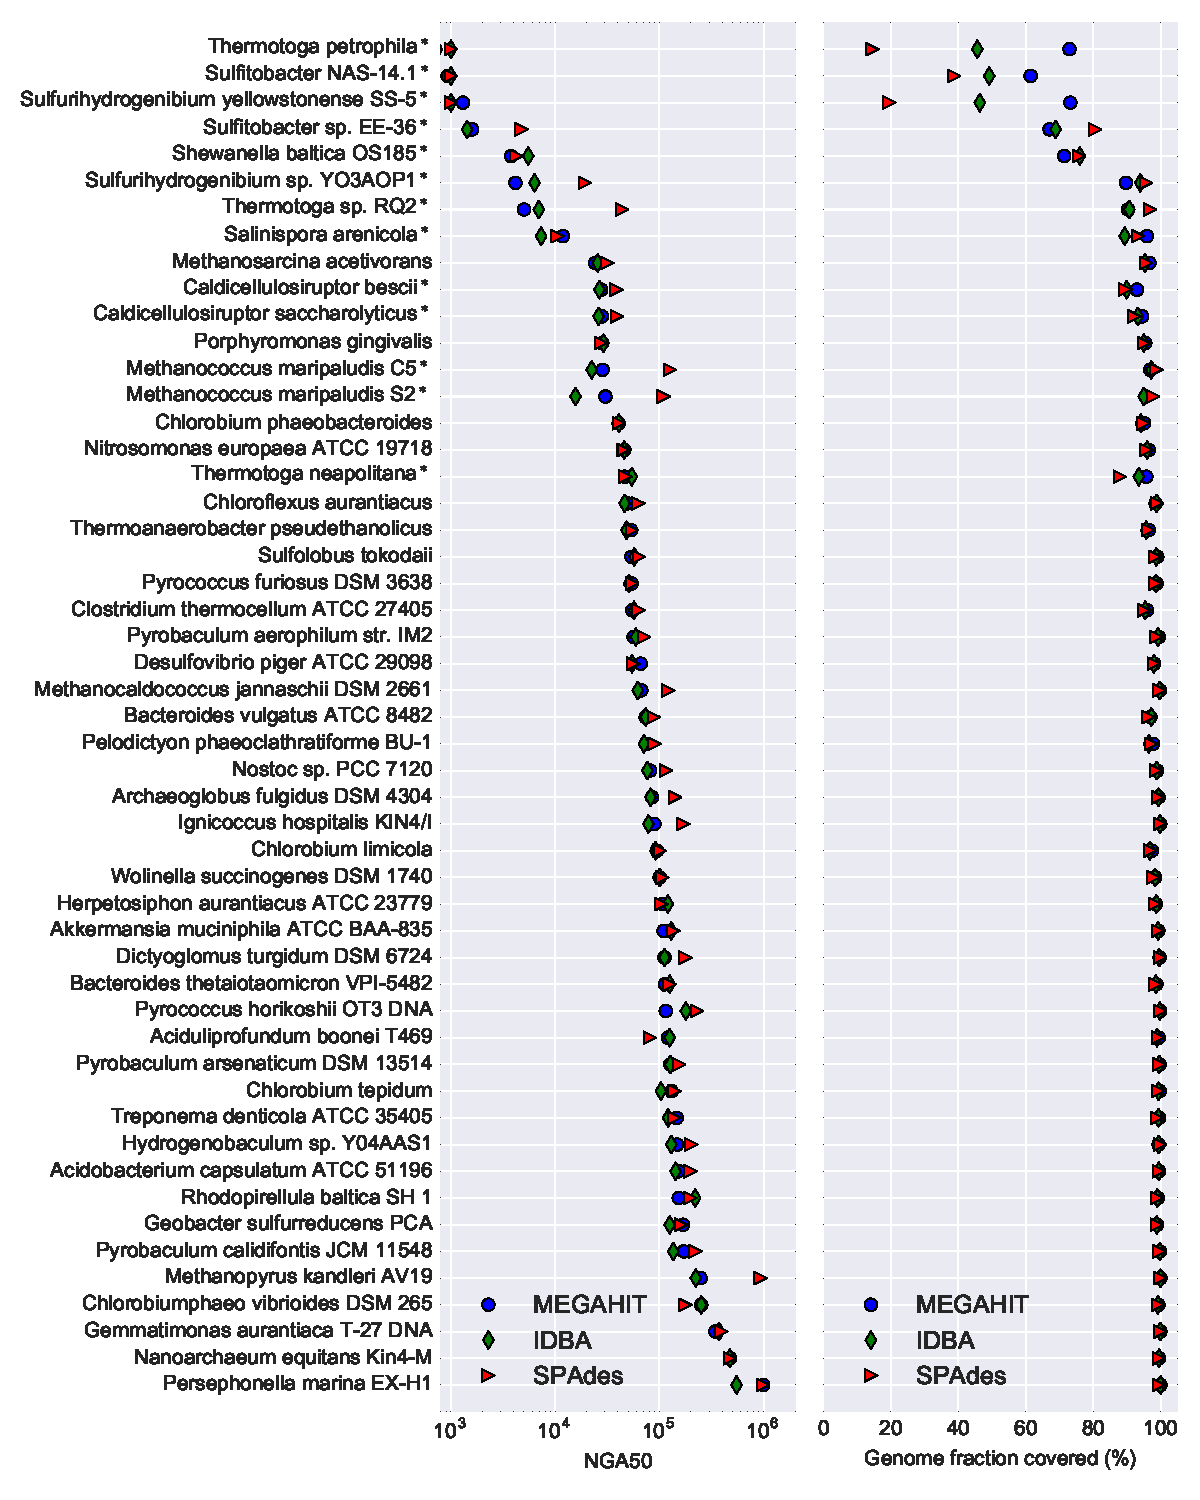
\includegraphics[width=\textwidth]{combined.pdf}  
\caption{NGA50 and genome fraction covered, by genome and assembler. A '*' after the name indicates the presence of at least one other genome with $>$ 2\% Jaccard similarity at k=31 in the community.  Where NGA50 cannot be calculated due to poor coverage, a marker is placed at 1kb.}
\label{fig:nga50}
\end{figure}

\newpage

\subsection*{Individual genome statistics vary widely in the assemblies.}

%The NGA50 for a particular genome in a metagenome is the minimum
%contig size at which 50\% of that genome is covered by aligned contigs.
We computed the NGA50 for each individual genome and assembly in order
to compare assembler performance on genome recovery (see left panel of
Figure~\ref{fig:nga50}).  The NGA50 statistics for individual genomes
vary widely, but there are consistent assembler-specific trends: IDBA
yields the lowest NGA50 for 28 of the 51 genomes, while MetaSPAdes yields
the highest NGA50 for 32 of the 51 genomes.

We also evaluated aligned coverage per genome for each of the three
assemblies (right panel, Figure~\ref{fig:nga50}).  We found that 13
of the 51 genomes were missing 5\% or more of bases in at least one
assembly, despite all 51 genomes having 99\% or higher read- and
51-mer coverage.

There are 12 genomes with k=31 Jaccard similarity greater than 2\% to
other genomes in the community, and these (denoted by '*' after the
name) typically had lower NGA50 and aligned coverage numbers than
other genomes.  In particular, these constituted 12 of the 13 genomes
missing 5\% or more of their content, and the lowest eight NGA50 numbers.

\subsection*{Longer contigs are less likely to be chimeric.}

\begin{table}[!h]
\centering
\caption{Chimeric contigs by contig length.}
\begin{tabular}{|l|c|c|c|}\hline
\textbf{Assembly} & \textbf {$>$ 50kb} & \textbf {$>$ 5kb} & \textbf{$>$ 500 bp}
\\ \hline

IDBA         & 0 & 1 & 7 (0.06\%) \\
MEGAHIT      & 1 & 4 & 14 (0.13\%) \\ 
MetaSPAdes       & 0 & 3 & 30 (0.48\%) \\
\hline

\end{tabular}
\label{table:contig-chimera}

\end{table}

% CTB ``it would be interesting to know what genes chimeric contigs...'' JG
% CTB JG: correlation b/t NGA50 and Jaccard?

Chimerism is the formation of contigs that include sequence from
multiple genomes.  We evaluated the rate of chimerism in contigs at
three different contig length cutoffs: 500bp, 5kb, and 50kb
(Table~\ref{table:contig-chimera}).  We found that the percentage of
contigs that match to the genomes of two or more different species
drop as the minimum contig size increases, to the point where only the
MEGAHIT assembly had a single chimeric contig longer than 50kb.
Overall, chimeric misassemblies were rare, with no assembler
generating more than 30 chimeric contigs out of thousands of total
contigs.

\subsection*{The unmapped reads contain strain variants of reference genomes.}

% number taken from unmapped-qc-to-ref.


% unmapped-qc-to-ref.fq:
% 4773066.0 total reads
% unmapped-qc-to-ref-rm.fq
%14674021

% >>> float(7494946 + 117005) / 108942761
% 0.06987110414798464
% >>> float(7494946 + 117005)
% 7611951.0

\begin{table}[t]
\caption{GenBank genomes detected in assembly of unmapped reads}
\centering
\begin{tabular}{|c|l|}
\hline

\textbf{match}& \textbf{GenBank genome} \\ [0.5ex] % inserts table %heading
44.1\% & {\em \small Fusobacterium sp.} OBRC1 \\
\hline
23.0\% & {\em \small P. ruminis strain} ML2 \\
\hline
18.2\% & {\em \small Thermus thermophilus} HB8 \\
\hline
7.7\% & {\em \small P. ruminis strain} CGMCC \\
\hline
8.2\% & {\em \small Enterococcus faecalis} M7 \\
\hline
7.3\% & {\em \small F. nucleatum} 13\_3C  \\
\hline
3.7\% & {\em \small F. nucleatum subsp. polymorphum} \\
\hline
2.9\% & {\em \small Fusobacterium hwasookii} \\
\hline
1.0\% & {\em \small E. coli isolate} YS \\
\hline
1.7\% & {\em \small F. nucleatum subsp. polymorphum}, alt. \\
\hline
1.9\% & {\em \small F. nucleatum subsp. vincentii} \\
\hline

\end{tabular}
\label{table:gather}
\end{table}

Approximately 4.8 million reads (4.4\%) from the QC data set did not
map anywhere in the reference provided by the authors of \cite{podar}.
We extracted and assembled these reads in isolation using MEGAHIT,
yielding 6.5 Mbp of assembly in 1711 contigs $>$ 500bp in length.  We
then did a k-mer inclusion analysis of this assembly against all of
the GenBank genomes at k=31, and estimated the fraction of the k-mers
that belonged to different species (Table~\ref{table:gather}). We find
that 51.1\% of the k-mer content of these contigs positively match to
a genome present in GenBank but not in the reference metagenome.

To verify these assignments, we aligned the MEGAHIT assembly of
unmapped reads to the GenBank genomes in Table~\ref{table:gather} with
NUCmer using ``loose'' alignment criteria. We found that 1.78 Mbp of
the contigs aligned at 99\% identity or better to these GenBank
genomes.  We also confirmed that, as expected, there are no matches in
this assembly to the full updated reference metagenome.

We note that all but the two {\em P. ruminis} matches and the {\em
  E. coli} isolate YS are strain variants of species that are part of
the defined community but are not completely present in the reads (see
Table~\ref{table:genomes_uncovered-analysis}).  For {\em
  Proteiniclasticum ruminis}, there is no closely related species in
the mock community design, and very little of the MEGAHIT assembly
aligns to known {\em P. ruminis} genomes at 99\%.  However, there are
many alignments to {\em P. ruminis} at 94\% or higher, for
approximately 2.73 Mbp total.  This suggests that the unmapped reads
contain at least some data from a novel species of {\em
  Proteiniclasticum}; this matches the observation in \cite{podar} of
a contaminating genome from an unknown {\em Clostridium} spp., as at the time
there was no {\em P. ruminis} genome.

\section*{Discussion}

\subsection*{Assembly recovers basic content sensitively and accurately.}

All three assemblers performed well in assembling contigs from the
content that was fully present in reads and k-mers.  After length filtering,
all three assemblies contained more than 95\% of the reference
(Table~\ref{table:contig-coverage}); even with removal of secondary
alignments, more than 87\% was recovered by each assembler
(Table~\ref{table:contig-accuracy}). About half the constituent genomes had
an NGA50 of 50kb or higher (Figure~\ref{fig:nga50}),
which, while low for current Illumina single-genome sequencing,
is sufficient to recover operon-level relationships for many genes.

% (Mention genes / prokka analysis.)

% CTB do we want to include sourmash comparison matrix?

\subsection*{The presence of multiple closely related genomes confounds assembly.}

In agreement with CAMI, we also find that the presence of closely related
genomes in the metagenome causes loss of assembly \cite{CAMI}.  This is
clearly shown by Figure~\ref{fig:nga50}, where 12 of the bottom 14
genomes by NGA50 (left panel) also exhibit poor genome recovery by
assembly (right panel).  Interestingly, different assemblers handle
this quite differently, with e.g. MetaSPAdes failing to recover
essentially any of {\em Thermotoga petrophila}, while MEGAHIT recovers
73\%.  The presence of nearby genomes is an almost perfect predictor
that one or more assembler will fail to recover 5\% or more - of the
13/51 genomes for which less than 95\% is recovered, 12 of them have
close genomes in the community.  Interestingly, very little similarity
is needed - all genomes with Jaccard similarity of 2\% or higher at k=31
exhibit these problems.

The {\em Shewanella baltica} OS185 genome is a good example: there
are two strain variants, OS185 and OS223, present in the defined
community.  Both are present at more than 99\% in the reads, and more
than 98\% in 51-mers, but only 75\% of {\em S. baltica} OS185 and 50\%
of {\em S. baltica} OS223 are recovered by assemblers.  This is a
clear case of ``strain confusion'' where the assemblers simply fail to
output contigs for a substantial portion of the two genomes.

Another interest of this study was to examine cross-species chimeric
assembly, in which a single contig is formed from multiple genomes.
In Table~\ref{table:contig-chimera}, we show that there is relatively
little cross-species chimerism.  Surprisingly, what little is present is
length-dependent: longer contigs are less likely to be chimeric.  This
might well be due to the same ``strain confusion'' effect as above,
where contigs that share paths in the assembly graphs are broken in twain.

\subsection*{MEGAHIT performs best by several metrics.}

MEGAHIT is clearly the most efficient computationally, outperforming
both MetaSPAdes and IDBA in memory and time
(Table~\ref{table:time-memory}).  The MEGAHIT assembly also included
more of the reads than either IDBA or MetaSPAdes, and omitted only 0.4\%
more of the unique 51-mers from the reads than IDBA.  MEGAHIT covered
more of the reference genome with both loose and strict alignments
(Table~\ref{table:contig-coverage} and
Table~\ref{table:contig-accuracy}), with little duplication.  This is
clearly because of MEGAHIT's generally superior performance in recovering the
genomes of closely related strains (Figure~\ref{fig:nga50}, right
panel).  The sum ``fraction of genome recovered'' is arguably the most
important measure of a metagenome assembler (see \cite{Vollmers2017}
in particular) and here MEGAHIT excels for individual genomes even in
the presence of strain variation.

% @CTB reference Nature foo strain foo.


When comparing details of sequence recovery between the assemblers,
the assembly content differs by only a small amount when loose
alignments are allowed: all three assemblers miss more content
(approximately 2.5\% of the reference) than they generate uniquely
(1.7\% or less).  In addition to preferring no one assembler over any
other, this suggests that combining assemblies may have little value
in terms of recovering additional metagenome content.

\subsection*{The missing reference may be present in strain variants of the intended species.}

Several individual genomes are missing in measurable portion from the
QC reads (Table~\ref{table:genomes_uncovered-analysis}), and many QC
reads (4.4\% of 108m) did not map to the full reference metagenome.
These appear to be related issues: upon analysis of the unmapped reads
against GenBank, we find that many of the contigs assembled from the
unmapped reads can be assigned to strain variants of the species in
the mock community (Table~\ref{table:gather}).  This suggests that the
constructors of the mock community may have unintentionally included
strain variants of {\em Fusobacterium nucleatum}, {\em Thermus
  thermophilus} HB27, and {\em Enterococcus faecalis}; note that the
microbes used were sourced from the community rather than the ATCC
(M. Podar, pers.  communication).  In addition, we detect what may be
portions of a novel member of the {\em Proteiniclasticum} genus in the
assembly of these reads - this is likely the {\em Clostridium} spp. detected
through amplicon sequencing in \cite{podar}.

Without returning to the original DNA samples, it is impossible to
conclusively confirm that unintended strains were used in the
construction of the mock community.  In particular, our analysis is
dependent on the genomes in GenBank: the genomes we detect in the
contigs are clearly closely related to GenBank genomes not in
the reference metagenome, based on k-mer analysis and
contig alignment.  However, GenBank is unlikely to contain the exact
genomes of the actually included strain variants, rendering conclusive
identification impossible.

\section*{Conclusions}


Overall, assembly of this mock community works well, with good
recovery of known genomic sequence for the majority of genomes.  All
three assemblers that we evaluated recover similar amounts of most
genomic sequence, but (recapitulating several other studies \cite{CAMI,Vollmers2017,metag_one})
MEGAHIT is computationally the most efficient of the three.
We note that assembly
resolves substantial portions of several previously undetected strain
variants, as well as recovering a substantial portion of a novel
{\em Proteiniclasticum} spp. that was detected via amplicon analysis
in \cite{podar}, suggesting that assembly is a useful complement to amplicon
or reference-based analyses.

The presence of closely related strains is a major confounder of
metagenome assembly, and causes assemblers to drop considerable
portions of genomes that (based on read mapping and k-mer inclusion)
are clearly present.  In this relatively simple community, this strain
confusion is present but does not dominate the assembly.  However,
real microbial communities are likely to have many closely related
strains and any resulting loss of assembly would be hard to detect in
the absence of good reference genomes.  While high polymorphism rates
in e.g. animal genomes are known to cause duplication or loss of
assembly, some solutions have emerged that make use of assumptions of
uniform coverage and diploidy \cite{Kim2007}.  These solutions cannot
however be transferred directly to metagenomes, which have unknown
abundance distributions and strain content.

An additional concern is that metagenome assemblies are often
performed after pooling data sets to increase coverage
(e.g. \cite{Sharon2012,Hu2016}); this pooled data is more likely to
contain multiple strains, which would then in turn adversely affect
assembly of strains.  This may not be resolvable within the current
paradigm of assembly, which focuses on outputting linear assemblies
that cannot properly represent strain variation.  The human genomics
community is moving towards using {\em reference graphs}, which can
represent multiple incompatible variants in a single data structure
\cite{paten2017genome}; this approach, however, requires high-quality
isolate reference genomes, which are generally unavailable for
environmental microbes.

Long read sequencing (and related technologies) will undoubtedly help
resolve strain variation in the future, but even with highly accurate
long-read sequencing, current sequencing depth is still too low to
resolve deep environmental metagenomes \cite{Sharon2015,White2016}.
It is unclear how well long error-prone reads (such as those output by
Pacific Biosciences SMRT \cite{Eid2009} and Oxford Nanopore
instruments \cite{Cherf2012}) will perform on complex metagenomes:
with high error rates, deep coverage of each individual genome is
required to achieve accurate assembly, and this may not be easily
obtainable for complex communities.  Single-molecule barcoding
(e.g. 10X Genomics \cite{Moss125211}) and HiC approaches
\cite{SmukowskiHeil150722} show promise but these remain untested on
well-defined complex communities and are still challenged by the
complexity of complex environmental metagenomes; see
\cite{Burton2014,Marbouty2014,Beitel2014}.

Much of our analysis above depends on having a high-quality ``mock''
metagenome.  While computationally constructed synthetic communities
and computational ``spike-ins'' to real data sets can provide valuable
controls (e.g. see \cite{metag_one} and \cite{ahowe2014}) we strongly
believe that standardized communities constructed {\em in vitro} and
sequenced with the latest technologies are critical to the evaluation
of both canonical and emerging tools, e.g. efforts such as
\cite{Brown2017}. From the perspective of tool evaluation, we must
disagree somewhat with Vollmers et al. \cite{Vollmers2017}: good
metagenome tool evaluation necessarily depends on mock communities
that are as realistic as we can make them.  Likewise, from the
perspective of bench biologists, actually sequencing real DNA is
critical because it can evaluate confounding effects such as kit
contamination \cite{Salter2014}.  Large-scale studies of computational
approaches systematically applied to mock communities such as CAMI
\cite{CAMI} can then provide fair comparisons of entire toolchains
(wet + dry) applied to these mock communities.

% CTB didn't mesaure N50, error rates, etc.
% CTB size cutoff for recovery / binning / 2kb on figure!!

We omitted two important questions in this study: binning and choice
of parameters.  We chose not to evaluate genome binning because most
binning strategies either operate post-assembly (see
e.g. \cite{laczny2017busybee}), in which case the challenges with
assembly discussed above will apply; or require multiple samples
(e.g. \cite{Cleary2015}), which we do not have.  We also chose to use
only default parameters with all three assemblers, for two reasons.
First, we are not aware of any widely used automated approaches for
determining the ``best'' set of parameters or evaluating the output,
other than those integrated into the assemblers themselves
(e.g. choice of k-mer sizes), and absent such guidance we do not feel
comfortable blessing any particular set of parameters; here the choice
of default parameters is parsimonious.  Second, any parameter
exploration pipeline would not only need to be automated but would
need to run multiple assemblies, whose time and resource usage should
be measured; in this case, any comparison based on
runtime of the parameter choice pipeline should naturally favor MEGAHIT
because of its advantage in computational efficiency.

\subsection*{Author contributions}

SA, LI and CTB developed, tested, and executed the analytical pipeline.
SA and CTB created the tables and figures and wrote the paper.

\subsection*{Competing interests}
No competing interest to our knowledge.

\subsection*{Grant information}
This work is funded by
Gordon and Betty Moore Foundation Grant GBMF4551 and
NIH NHGRI R01 grant HG007513-03, both to CTB.

\subsection*{Acknowledgments}
We thank Michael R. Crusoe and Phillip T. Brooks for input on analysis
and pipeline development.  We thank Migun Shakya, Mircea Podar, Jiarong Guo,
Harald R. Gruber-Vodicka, Juliane Wippler, Krista Ternus, and Stephen
Turner for valuable comments on drafts of this manuscript.

{\small\bibliographystyle{unsrtnat} \bibliography{references}}

\bigskip
% References can be listed in any standard referencing style that uses a numbering system
% (i.e. not Harvard referencing style), and should be consistent between references within
% a given article.

% Reference management systems such as Zotero provide options for exporting bibliographies as Bib\TeX{} files. Bib\TeX{} is a bibliographic tool that is used with \LaTeX{} to help organize the user's references and create a bibliography. This template contains an example of such a file, \texttt{references.bib}, which can be replaced with your own. Use the \verb|\cite| command  to create in-text citations, like this .


% See this guide for more information on BibTeX:
% http://libguides.mit.edu/content.php?pid=55482&sid=406343

% For more author guidance please see:
% http://f1000research.com/author-guidelines


% When all authors are happy with the paper, use the 
% ‘Submit to F1000Research' button from the menu above
% to submit directly to the open life science journal F1000Research.

% Please note that this template results in a draft pre-submission PDF document.
% Articles will be professionally typeset when accepted for publication.

% We hope you find the F1000Research Overleaf template useful,
% please let us know if you have any feedback using the help menu above.



\end{document}
